% =============================================================
% Experiment 1
% Clipping and Clamping Circuits using Diodes
%
% Required packages in the master document preamble:
%   amsmath, amssymb, graphicx, circuitikz, pgfplots, booktabs,
%   enumitem, siunitx, hyperref
%   \pgfplotsset{compat=1.17}
% =============================================================

\chapter{Clipping and Clamping Circuits using Diodes}
\label{sec:expt1}

\section{Aim}
\begin{enumerate}[label=(\roman*)]
	\item To study the operation of series and shunt diode clipping circuits and to observe the effect of biasing on the clipping level.
	\item To study the operation of positive and negative diode clamping circuits.
	\item To design clipper and clamper circuits for specified output requirements.
	\item To verify, using a DSO, that the observed waveforms agree with the theoretically predicted transfer characteristics.
\end{enumerate}
\section{Pre-Lab Exercise}
Before performing the experiment, simulate the circuits and verify the designs using LTspice or any other circuit simulation software. 
\section{Equipment/Components Required}
\begin{table}[h!]
	\centering
	\begin{tabular}{@{}cll@{}}
		\toprule
		S.No. & Equipment/Component & Specification \\
		\midrule
		1 & Digital Storage Oscilloscope & 2-channel, 20--50\,MHz bandwidth \\
		2 & Function Generator\footnote{Instead of function generator, a step-down transformer may also be used to apply the input signal, which will then be a 50 Hz sine wave.} & Sine wave, 1\,Hz -- 1\,MHz \\
		3 & Regulated DC Power Supply & 0--30\,V \\
		4 & Silicon diode & 1N4007 (or equivalent), 2 nos. \\
		5 & Zener diodes & $V_z$ = 5.6 V, 2 nos. \\
		6 & Resistors & 1\,k$\Omega$ -- 100\,k$\Omega$ \\
		7 & Capacitors & 1\,$\mu$F -- 10\,$\mu$F \\
		8 & Breadboard and connecting wires & -- \\
		\bottomrule
	\end{tabular}
	\caption{Equipment and component list.}
\end{table}

\section{Theory}

Diode clipping and clamping circuits exploit the nonlinear, near-ideal-switch behaviour of a $p$--$n$ junction diode to reshape a waveform. A \emph{clipper} removes (clips) a portion of the input waveform above and/or below a reference level, while a \emph{clamper} shifts the entire waveform up or down without altering its shape, thereby changing its DC reference level.

Throughout this document, the diode is modelled as an ideal switch in series with a cut-in voltage $V_F \approx 0.7\,\text{V}$ (silicon) and a forward resistance $R_f \approx 0$; the reverse resistance is assumed infinite. 

\subsection{Clipping Circuits}

\paragraph{(a) Series (Half-Wave) Clipper.}\footnote{This circuit need not be assembled and tested. This is presented here for completeness.}
Figure~\ref{fig:series_clipper} shows a series diode clipper. The diode conducts only when $v_{in}$ forward-biases it, so the circuit passes only one half-cycle of the input to the output. The output voltage across the resistance $R_L$ will be $v_{in}(t)-V_F$, for $v(t)>0$, and $0\, \text{V}$ for $v(t)<0$.

\begin{figure}[htbp]
	\centering
	\begin{circuitikz}[american, scale=0.8, line width = 0.8pt]
		\draw
		(0,0) to[sinusoidal voltage source, l=$v_{in}(t)$] (0,3)
		(0,3) to[short] (1,3)
		(1,3) to[D, l=$D$, *-*] (3,3)
		(3,3) to[R, l=$R_L$, *-*] (3,0)
		(3,0) to[short] (0,0)
		;
		\draw (3,3) to[short, -o] (3.7,3) node[right]{$v_{out}(t)$};
		\draw (3,0) to[short, -o] (3.7,0) node[right]{};
		\draw (0,0) node[ground]{};
	\end{circuitikz}
	\caption{Series (half-wave) diode clipper. The diode conducts on the positive half-cycle and passes it to $R_L$; the negative half-cycle is clipped.}
	\label{fig:series_clipper}
\end{figure}

\paragraph{(b) Shunt (Parallel) Clipper -- Positive Clipper.}
Figure~\ref{fig:ShuntPosClipperCkt} shows a shunt clipper with the diode across the output. Whenever $v_{in} > V_F (\approx 0.7\ \text{V})$, the diode conducts and clips the output at $V_F$. For $v_{in}(t) < V_F$, the diode is OFF and $v_{out} = v_{in}\frac{R_L}{R_L+R}$. If $R_L \gg R$, $v_{out}\approx v_{in}$, during the negative cycle . The waveforms expected are as given in Fig.~\ref{fig:wavePosClipper}. 


The positive portion of the input waveform is clipped off, hence the name positive clipper.
\paragraph{(c) Shunt (Parallel) Clipper -- Negative Clipper.}
Figure~\ref{fig:ShuntNegClipperCkt} shows a shunt negative clipper with the diode across the output, placed in the opposite polarity compared to the positive clipper. Whenever $v_{in}(t) < -V_F$, the diode conducts and clamps the output near $-V_F$; for $v_{in}(t) > -V_F$, the diode is OFF and $v_{out} = v_{in}\dfrac{R_L}{R_L+R}$. If $R_L \gg R$, $v_{out}\approx v_{in}$, during the positive cycle. The waveforms expected are as given in Fig.~\ref{fig:NegClipperWaves}. 

The negative portion of the input waveform is clipped off, hence the name negative clipper.
\paragraph{(d) Biased Clippers.}
A DC bias source $V_R$ in series with the diode (Figure~\ref{fig:biasedClippers}) shifts the clipping level from $V_F$ to $(V_R + V_F)$ or $(V_R - V_F)$, depending on polarity. This allows the clipping level to be set anywhere on the waveform. There are two ways to achieve the biasing. One is to provide a direct dc source. The other is to use a Zener diode or series combination of diodes to achieve the bias level.

Fig.~\ref{fig:biasedPosClipperDc} shows a biased positive clipper with a dc bias. Fig.~\ref{fig:biasedPosClipperZener} shows the implementation with a Zener diode. The clipping levels are $V_R+V_F$ and $V_Z+V_F$ respectively. Fig.~\ref{fig:biasedPosClipperWaves} shows the sample waveforms. 
%\begin{figure}[htbp]
%	\centering
%	\begin{circuitikz}[american, scale=1.0, line width=0.8pt]
%		\draw
%		(0,0) to[sinusoidal voltage source, l=$v_{in}(t)$] (0,3)
%		(0,3) to[R, l=$R$, *-*] (3,3)
%		(3,3) to[short] (4,3)
%		(3,3) to[D, l=$D$, *-*] (3,1.5)
%		(3,1.5) to[battery1, l=$V_R$] (3,0)
%		(3,0) to[short, *-*] (0,0)
%		;
%		\draw (4,3) to[short, -o] (4.7,3) node[right]{$v_{out}(t)$};
%		\draw (3,0) to[short, -o] (4.7,0) node[right]{};
%		\draw (0,0) node[ground]{};
%	\end{circuitikz}
%	\caption{Biased shunt clipper. Output is clipped at approximately $V_R + V_F$.}
%	\label{fig:biased_clipper}
%\end{figure}

In a similar way, a \textbf{Biased Negative Clipper} can be implemented by reversing the diode polarity. The figures~\ref{fig:biasedNegClipperDc} and \ref{fig:biasedNegClipperZener} show the circuit implementations.

The sample waveforms for the biased negative clipper are as shown in Fig.~\ref{fig:biasedNegClipperWaves}.


\paragraph{Double (Two-Level) Clipper or Slicer.}
Two diodes, oppositely poled and biased at $V_{R1}$ and $V_{R2}$, in parallel (Figure~\ref{fig:double_clipper}), clip both the positive peak above $(V_{R1}+V_F)$ and the negative peak below $-(V_{R2}+V_F)$, producing a trapezoidal output for a sinusoidal input of sufficient amplitude. If the amplitude of the sine wave is much larger compared to the clipping level, the output waveform approximates a square-wave. This circuit is also known as a `slicer'. 

Instead of DC biasing voltages, zener diodes can be used.
\subsubsection{Transfer Characteristics}
The transfer characteristics are graphs which plot the output (voltage) against the input (voltage). They give a visual indication of about the relationship between the input and the output. They also visualise which region of the operation of the circuit is linear. The transfer characteristics of the various clipper circuits are shown along with their respective circuit diagrams, in the section~\ref{sec:cktDiagramsClipper}. 

%\clearpage
\subsection{Clamping Circuits}

A clamper consists of a diode, a capacitor, and a resistor, arranged so that the capacitor charges (through the low forward resistance of the diode) to the peak of the input during one half-cycle and holds this charge (discharging slowly through $R_L$, with $R_LC \gg T$) during the rest of the cycle, thereby shifting the DC level of the waveform. It essentially `clamps' the input signal up or down by the peak voltage. It is also called a DC restorer.

Mathematically, for an input signal given by $v){in}(t) = V_m\sin(\omega t)$, the clamper output is $v_o(t)= \pm V_m + V_m\sin(\omega t)$.

\paragraph{(a) Negative Clamper.}
Figure~\ref{fig:neg_clamper} shows a negative clamper, which shifts the waveform downward so that its positive peak is clamped at (approximately) $0\,\text{V}$ (or at $V_F$, accounting for diode drop).


\paragraph{(b) Positive Clamper.}
Reversing the diode polarity (Figure~\ref{fig:pos_clamper}) clamps the negative peak of the waveform at approximately $0\,\text{V}$, shifting the entire waveform upward.


For an input sine wave of amplitude $V_m$, the steady-state clamped output ideally swings between:
\begin{align}
	\text{Negative clamper: } && v_{out} &\in [-2V_m + V_F,\; V_F], \label{eq:neg_clamp}\\
	\text{Positive clamper: } && v_{out} &\in [-V_F,\; 2V_m - V_F]. \label{eq:pos_clamp}
\end{align}
The time constant $R_L C$ must satisfy $R_L C \gg T$ (the input period) so that the capacitor voltage does not decay appreciably between successive charging peaks (poor choice of $R_L C$ leads to \emph{waveform tilt/sag}).
%\clearpage

\section{Design Example}
\begin{enumerate}[label=(\alph*)]
	\item Select the operating signal's frequency and amplitude, $V_m = 10\ \text{V}$ and $f = 100\ \text{Hz}$. 
	\item The series resistor R should not be too large or too small. $R_{min}$ is decided by the maximum current in the circuit. A typical value for R would be $1\ \text{k}\Omega$. Since $R_L\gg R$, $R_L \geq 100\ \text{k}\Omega$\footnote{For viewing on the DSO, $R_L$ may be removed, then $V_{out}$ would be same as $V_{in}$, since the input impedance of DSO is in $\text{M}\Omega$.  In practical circuits where the clipped waveform is applied as input to other circuits, $R_L$ represents the input impedance of those circuits.}. The output voltage peak then would be:
	\[
	V_{out,m}=\frac{V_mR_L}{R+R_L} = \frac{10\times 100\ \text{k}}{1\ \text{k}+100\ \text{k}} = 9.9 \ \text{V}
	\]
	 
	\item For a \textbf{biased clipper} required to clip at a level $V_{clip}<V_m$, select $V_R = V_{clip} - V_F$ using a potential divider from the DC supply, or a battery/regulated source directly. A Zener diode may also be chosen, as described earlier. Let $V_{clip} = 6.3\ \text{V}$. Then $V_R = V_{clip} - V_F\ =\ 6.3-0.7 = 5.6\ \text{V}$. In this case, either a dc voltage of $5.6\ \text{V}$ or a Zener diode of $V_Z=5.6\ \text{V}$ may be used as bias $V_R$.
	\item For a \textbf{clamper}, choose $C$ such that $R_L C \geq 10\,T$, where $T = 1/f$ is the period of the lowest input frequency to be used, so that the sag in output during discharge is limited to within an acceptable fraction (typically $< 5\%$) of $V_m$. For $f=100\ \text{Hz}$, $T=10\ \text{ms}$. Then, for $C = 1\ \mu F$ electrolytic:
	\[
	R_L C \geq 10\,T \Rightarrow R_L \geq \frac{10\times 10\times 10^{-3}}{1\times 10^{-6}}
	\]
	which yields:
	\[
	R_L\geq 100\ \text{k}\Omega
	\]
	%\item Choose $R_L$ in clampers large enough to limit diode conduction current to a safe value. 
	\item \textbf{Selection of diodes}: For input frequencies less than 1 kHz, line frequency diodes such as 1N4001 may be used. For higher frequencies, these slow diodes are to be replaced with faster signal diodes such as 1N4148.
\end{enumerate}
\section{Circuit Diagrams}
\subsection{Clipping Circuits}\label{sec:cktDiagramsClipper}
\subsubsection{Shunt Positive Clipper}
\begin{figure}[htbp]
	\centering
	%	
	%	% ---------- LEFT: circuit ----------
	\begin{subfigure}{0.52\textwidth}
		\centering
		\begin{circuitikz}[american, scale=0.75, line width=0.8pt]
			\draw
			(0,0) to[sinusoidal voltage source, l=$v_{in}(t)$] (0,3)
			(0,3) to[R, l=$R$, *-*] (4,3)
			(4,3) to[short] (6,3)
			(4,3) to[D, l=$D$, *-*, mirror] (4,0)
			(4,0) to[short, *-*] (0,0)
			(6,3) to[R, l=$R_L$, *-*] (6,0)
			(6,0) to[short] (4,0);
			\draw (6,3) to[short, -o] (6.7,3) node[right]{$v_{out}(t)$};
			\draw (6,0) to[short, -o] (6.7,0) node[right]{};
			\draw (0,0) node[ground]{};
		\end{circuitikz}
		\caption{Shunt positive clipper Circuit}
		\label{fig:ShuntPosClipperCkt}
			%	% ---------- Transfer chara----------
		\begin{subfigure}{0.52\textwidth}
			\centering
			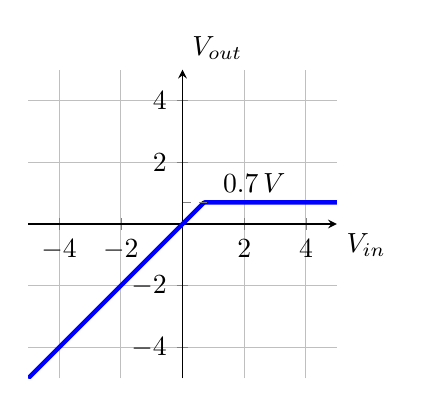
\begin{tikzpicture}
				\begin{axis}[
					axis lines=middle,
					xlabel={$V_{in}$},
					ylabel={$V_{out}$},
					xmin=-5, xmax=5,
					ymin=-5, ymax=5,
					grid=both,
					width=5.5cm, height=5.5cm,
					xlabel style={at={(ticklabel* cs:1)}, anchor=north west},
					ylabel style={at={(ticklabel* cs:1)}, anchor=south west},
					%title={\textbf{Positive Clipper}}
					]
					% V_out = min(V_in, 0)
					\addplot[ultra thick, blue, domain=-5:5, samples=200] {min(x, 0.7)};
					\draw[dashed, gray] (axis cs:0,0.7) -- (axis cs:1,0.7) node[above right, black] {$0.7\, \text{V}$};
				\end{axis}
			\end{tikzpicture}
			\caption{Transfer Characteristics}
			\label{fig:TransferCharaPosClipper}
		\end{subfigure}
	\end{subfigure}
	\hfill
	%	% ---------- RIGHT: stacked plots ----------
	\begin{subfigure}{0.4\textwidth}
		\centering
		%	
		\begin{tikzpicture}
			\begin{groupplot}[
				group style={
					group size=1 by 2,
					vertical sep=1.0cm,
				},
				width=7.5cm, height=5.0cm,
				axis lines=middle,
				xmin=-0.3, xmax=4.5,
				ymin=-6, ymax=6,
				xtick={0,2,4},
				xticklabels={$0$,$T$,$2T$},
				domain=0:4,
				samples=200,
				clip=false,
				]			
				% ---------- PANEL 1: INPUT ----------
				\nextgroupplot[
				ylabel={$v_{in}(t)$},
				ylabel style={
					at={(axis description cs:0,1)},  % top-left corner of the axis
					anchor=south,
					rotate=0,
				},
				ytick={5,-5},
				yticklabels={$V_m$,$-V_m$},
				]
				\addplot[thick, blue] {5*sin(deg(pi*x))};
				\draw[dashed, gray] (axis cs:0,5) -- (axis cs:4,5);
				\draw[dashed, gray] (axis cs:0,-5) -- (axis cs:4,-5);
				
				% ---------- PANEL 2: OUTPUT (clipped) ----------
				\nextgroupplot[
				ylabel={$v_{out}(t)$},
				ylabel style={
					at={(axis description cs:0,1)},  % top-left corner of the axis
					anchor=south,
					rotate=0,
				},
				ytick={0.7,-5},
				yticklabels={$0.7\,\text{V}$,$-V_m$},
				samples=400,
				]
				\addplot[thick, red] {min(5*sin(deg(pi*x)), 0.7)};
				\draw[dashed, gray] (axis cs:0,0.7) -- (axis cs:4,0.7);
				\draw[dashed, gray] (axis cs:0,-5) -- (axis cs:4,-5);			
			\end{groupplot}
		\end{tikzpicture}
		\caption{Positive clipper waveforms}
		\label{fig:wavePosClipper}	
	\end{subfigure}	
	\caption{Positive clipper circuit, input/output waveforms and transfer characteristics}
	\label{fig:PosClipper}
\end{figure}
\clearpage
\subsubsection{Shunt Negative Clipper}
\begin{figure}[htbp]
	\centering
	%	
	%	% ---------- LEFT: circuit ----------
	\begin{subfigure}{0.52\textwidth}
		\centering
		\begin{circuitikz}[american, scale=0.75, line width=0.8pt]
			\draw
			(0,0) to[sinusoidal voltage source, l=$v_{in}(t)$] (0,3)
			(0,3) to[R, l=$R$, *-*] (4,3)
			(4,3) to[short] (6,3)
			(4,3) to[D, l=$D$, *-*, invert] (4,0)
			(4,0) to[short, *-*] (0,0)
			(6,3) to[R, l=$R_L$, *-*] (6,0)
			(6,0) to[short] (4,0);
			\draw (6,3) to[short, -o] (6.7,3) node[right]{$v_{out}(t)$};
			\draw (6,0) to[short, -o] (6.7,0) node[right]{};
			\draw (0,0) node[ground]{};
		\end{circuitikz}
		\caption{Shunt negative clipper circuit}
		\label{fig:ShuntNegClipperCkt}
		
		\begin{subfigure}{0.52\textwidth}
			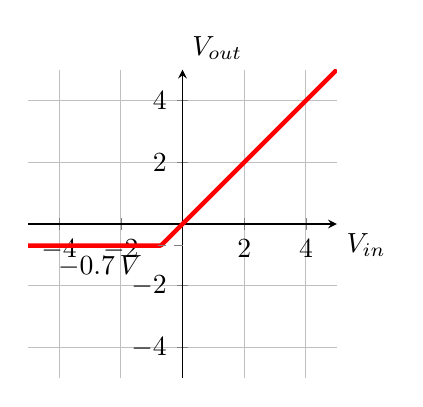
\begin{tikzpicture}
				\begin{axis}[
					axis lines=middle,
					xlabel={$V_{in}$},
					ylabel={$V_{out}$},
					xmin=-5, xmax=5,
					ymin=-5, ymax=5,
					grid=both,
					width=5.5cm, height=5.5cm,
					xlabel style={at={(ticklabel* cs:1)}, anchor=north west},
					ylabel style={at={(ticklabel* cs:1)}, anchor=south west},
					%title={\textbf{Negative Clipper}}
					]
					% V_out = max(V_in, 0)
					\addplot[ultra thick, red, domain=-5:5, samples=200] {max(x, -0.7)};
					\draw[dashed, gray] (axis cs:0,-0.7) -- (axis cs:-1,-0.7) node[below left, black] {$-0.7\, \text{V}$};
				\end{axis}
			\end{tikzpicture}
			\caption{Transfer characteristics of negative clipper}
			\label{fig:TransferCharaNegClipper}	
		\end{subfigure}
	\end{subfigure}
	\hfill
	%	% ---------- RIGHT: stacked plots ----------
	\begin{subfigure}{0.4\textwidth}
		\centering
		%	
		\begin{tikzpicture}
			\begin{groupplot}[
				group style={
					group size=1 by 2,
					vertical sep=1.0cm,
				},
				width=7.5cm, height=5cm,
				axis lines=middle,
				xmin=-0.3, xmax=4.5,
				ymin=-6, ymax=6,
				xtick={0,2,4},
				xticklabels={$0$,$T$,$2T$},
				domain=0:4,
				samples=200,
				clip=false,
				]
				
				% ---------- PANEL 1: INPUT ----------
				\nextgroupplot[
				ylabel={$v_{in}(t)$},
				ylabel style={
					at={(axis description cs:0,1)},  % top-left corner of the axis
					anchor=south,
					rotate=0,
				},
				ytick={5,-5},
				yticklabels={$V_m$,$-V_m$},
				]
				\addplot[thick, blue] {5*sin(deg(pi*x))};
				\draw[dashed, gray] (axis cs:0,5) -- (axis cs:4,5);
				\draw[dashed, gray] (axis cs:0,-5) -- (axis cs:4,-5);
				
				% ---------- PANEL 2: OUTPUT (clipped) ----------
				\nextgroupplot[
				ylabel={$v_{out}(t)$},
				ylabel style={
					at={(axis description cs:0,1)},  % top-left corner of the axis
					anchor=south,
					rotate=0,
				},
				ytick={-0.7,5},
				yticklabels={$-0.7\,\text{V}$,$V_m$},
				samples=400,
				]
				\addplot[thick, red] {max(-0.7, 5*sin(deg(pi*x)))};
				\draw[dashed, gray] (axis cs:0,-0.7) -- (axis cs:4,-0.7);
				\draw[dashed, gray] (axis cs:0,5) -- (axis cs:4,5);
				
			\end{groupplot}
		\end{tikzpicture}
		\caption{Negative clipper waveforms}
		\label{fig:NegClipperWaves}	
	\end{subfigure}
	%	
	\caption{Diode clipper circuit with input and output waveforms}
	\label{fig:NegClipper}
\end{figure}
\subsubsection{Biased Positive Clippers}
\begin{figure}[htbp]
	\centering
	\begin{subfigure}{0.42\textwidth}
		\centering
		\begin{circuitikz}[american, scale=1.0, line width=0.8pt]
			\draw
			(0,0) to[sinusoidal voltage source, l=$v_{in}(t)$] (0,3)
			(0,3) to[R, l=$R$, *-*] (3,3)
			(3,3) to[short] (4,3)
			(3,3) to[D, l=$D$, *-*] (3,1.5)
			(3,1.5) to[battery1, l=$V_R$] (3,0)
			(3,0) to[short, *-*] (0,0)
			;
			\draw (4,3) to[short, -o] (5,3) node[right]{$v_{out}(t)$};
			\draw (3,0) to[short, -o] (5,0) node[right]{};
			\draw (4.5,3) to [R, l=$R_L$, *-*] (4.5,0);
			\draw (0,0) node[ground]{};
		\end{circuitikz}
		\caption{Biased positive clipper with dc source bias}
		\label{fig:biasedPosClipperDc}
	\end{subfigure}
	\hfill
	\begin{subfigure}{0.42\textwidth}
		\centering
		\begin{circuitikz}[american, scale=1.0, line width=0.8pt]
			\draw
			(0,0) to[sinusoidal voltage source, l=$v_{in}(t)$] (0,3)
			(0,3) to[R, l=$R$, *-*] (3,3)
			(3,3) to[short] (4,3)
			(3,3) to[D, l=$D$, *-*] (3,1.5)
			(3,1.5) to[zzDo, l=$V_Z$, invert] (3,0)
			(3,0) to[short, *-*] (0,0)
			;
			\draw (4,3) to[short, -o] (5,3) node[right]{$v_{out}(t)$};
			\draw (3,0) to[short, -o] (5,0) node[right]{};
			\draw (4.5,3) to [R, l=$R_L$, *-*](4.5,0);
			\draw (0,0) node[ground]{};
		\end{circuitikz}
		\caption{Biased positive clipper with Zener diode as bias}
		\label{fig:biasedPosClipperZener}
	\end{subfigure}
	\caption{Biased positive clipper configurations}
	\label{fig:biasedClippers}
\end{figure}
\begin{figure}[htbp]
	\centering
	\begin{subfigure}{0.4\textwidth}
		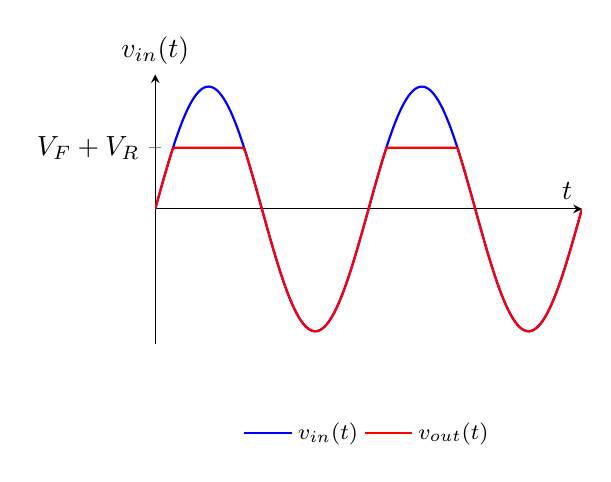
\begin{tikzpicture}
			\begin{axis}[
				width=7cm, height=5cm,
				xlabel={$t$}, 
				axis lines=middle,
				ymin=-2.2, ymax=2.2,
				ylabel={$v_{in}(t)$},
				ylabel style={
					at={(axis description cs:0,1)},  % top-left corner of the axis
					anchor=south,
					rotate=0,
				},
				xtick=\empty, ytick={1},
				yticklabels={$V_F+V_R$},
				domain=0:2, samples=200,
				legend style={draw=none, font=\footnotesize, at={(0.5,-0.25)}, anchor=north, legend columns=2}
				]
				\addplot[blue, thick] {2*sin(360*x)};
				\addlegendentry{$v_{in}(t)$}
				\addplot[red, thick] {min(2*sin(360*x), 1)};
				\addlegendentry{$v_{out}(t)$}
			\end{axis}
		\end{tikzpicture}
		\caption{Input and output waveforms for the biased positive clipper of Figure~\ref{fig:biasedPosClipperDc}: the output is flattened above $V_F+V_R$.}
		\label{fig:biasedPosClipperWaves}
	\end{subfigure}
	\hfill
	\begin{subfigure}{0.4\textwidth}
		\centering
		% --- BIASED POSITIVE (POSITIVE LEVEL +2V) ---
		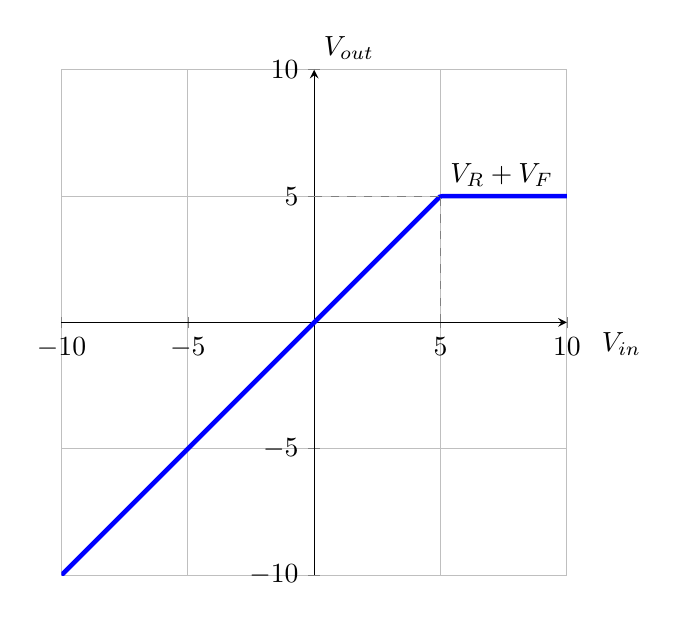
\begin{tikzpicture}
			\begin{axis}[
				axis lines=middle,
				xlabel={$V_{in}$},
				ylabel={$V_{out}$},
				xmin=-10, xmax=10,
				ymin=-10, ymax=10,
				grid=both,
				width=8cm, height=8cm,
				xlabel style={at={(ticklabel* cs:1.05)}, anchor=north west},
				ylabel style={at={(ticklabel* cs:1)}, anchor=south west},
				%title={\textbf{Biased Positive ($V_R = +2\text{V}$)}}
				]
				% Clipping behavior
				\addplot[ultra thick, blue, domain=-10:10, samples=200] {min(x, 5)};
				% Reference Guide Lines
				\draw[dashed, gray] (axis cs:5,0) -- (axis cs:5,5) node[above right, black] {$V_R+V_F$};
				\draw[dashed, gray] (axis cs:0,5) -- (axis cs:5,5);
			\end{axis}
		\end{tikzpicture}
		\caption{Transfer characteristics of biased positive clipper with clipping level at ($V_R+V_F)$}
		\label{fig:TransferCharaBiasPosClipperPosLevel}
	\end{subfigure}
	\caption{Biased positive clipper waveforms and transfer characteristics for a positive clipping level}
\end{figure}
The clipping level is moved to negative, by reversing the bias voltage $V_R$ in Fig.~\ref{fig:biasedPosClipperDc}. However, the same effect cannot be achieved through the circuit in Fig.~\ref{fig:biasedPosClipperZener} by reversing the Zener.
\begin{figure}[htbp]
	\centering
		\begin{subfigure}{0.4\textwidth}
		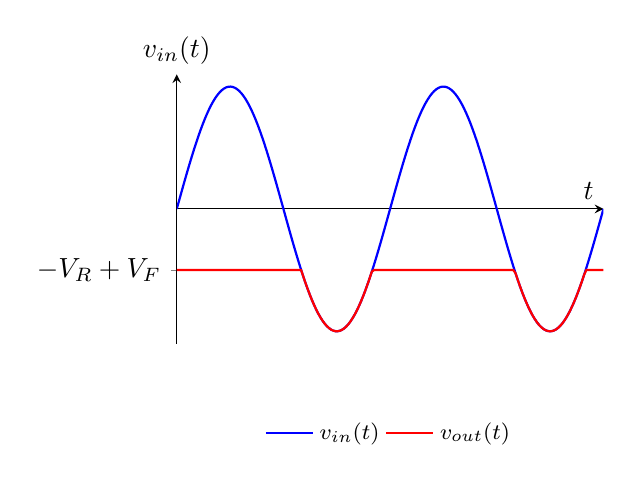
\begin{tikzpicture}
			\begin{axis}[
				width=7cm, height=5cm,
				xlabel={$t$}, 
				axis lines=middle,
				ymin=-2.2, ymax=2.2,
				ylabel={$v_{in}(t)$},
				ylabel style={
					at={(axis description cs:0,1)},  % top-left corner of the axis
					anchor=south,
					rotate=0,
				},
				xtick=\empty, ytick={-1},
				yticklabels={$-V_R+V_F$},
				domain=0:2, samples=200,
				legend style={draw=none, font=\footnotesize, at={(0.5,-0.25)}, anchor=north, legend columns=2}
				]
				\addplot[blue, thick] {2*sin(360*x)};
				\addlegendentry{$v_{in}(t)$}
				\addplot[red, thick] {min(2*sin(360*x), -1)};
				\addlegendentry{$v_{out}(t)$}
			\end{axis}
		\end{tikzpicture}
		\caption{Input and output waveforms for the biased positive clipper of Figure~\ref{fig:biasedPosClipperDc}, with $-V_R$: the output is flattened above $-V_R+V_F$.}
		\label{fig:biasedPosClipperNegLevelWaves}
	\end{subfigure}
	\hfill
	\begin{subfigure}{0.4\textwidth}
			% --- BIASED POSITIVE (NEGATIVE LEVEL -2V) ---
		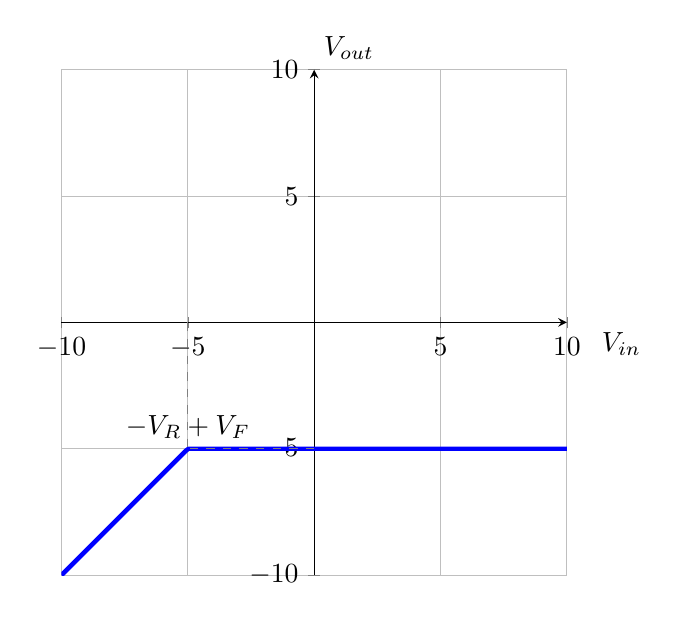
\begin{tikzpicture}
			\begin{axis}[
				axis lines=middle,
				xlabel={$V_{in}$},
				ylabel={$V_{out}$},
				xmin=-10, xmax=10,
				ymin=-10, ymax=10,
				grid=both,
				width=8cm, height=8cm,
				xlabel style={at={(ticklabel* cs:1.05)}, anchor=north west},
				ylabel style={at={(ticklabel* cs:1)}, anchor=south west},
			%	title={\textbf{$V_R = -2\text{V}$}}
				]
				% Clipping behavior
				\addplot[ultra thick, blue, domain=-10:10, samples=200] {min(x, -5)};
				% Reference Guide Lines
				\draw[dashed, gray] (axis cs:-5,0) -- (axis cs:-5,-5) node[above, black] {$-V_R+V_F$};
				\draw[dashed, gray] (axis cs:0,-5) -- (axis cs:-5,-5);
			\end{axis}
		\end{tikzpicture}
		\caption{Transfer characteristics of biased positive clipper with a negative clipping level}
		\label{fig:TransferCharaBiasPosClipperNegLevel}
	\end{subfigure}
	\caption{Waveforms and transfer characteristics of biased positive clipper with a negative clipping level}
\end{figure}
\clearpage
\subsubsection{Biased Negative Clippers}
\begin{figure}[htbp]
	\centering
	\begin{subfigure}{0.4\textwidth}
		\centering
		\begin{circuitikz}[american, scale=1.0, line width=0.8pt]
			\draw
			(0,0) to[sinusoidal voltage source, l=$v_{in}(t)$] (0,3)
			(0,3) to[R, l=$R$, *-*] (3,3)
			(3,3) to[short] (4,3)
			(3,3) to[D, l=$D$,invert, *-*] (3,1.5)
			(3,1.5) to[battery1, invert, l=$V_R$] (3,0)
			(3,0) to[short, *-*] (0,0)
			;
			\draw (4,3) to[short, -o] (5,3) node[right]{$v_{out}(t)$};
			\draw (3,0) to[short, -o] (5,0) node[right]{};
			\draw (4.5,3) to [R, l=$R_L$, *-*] (4.5,0);
			\draw (0,0) node[ground]{};
		\end{circuitikz}
		\caption{Biased negative clipper with dc source bias.}
		\label{fig:biasedNegClipperDc}
	\end{subfigure}
	\hfill
	\begin{subfigure}{0.4\textwidth}
		\centering
		\begin{circuitikz}[american, scale=1.0, line width=0.8pt]
			\draw
			(0,0) to[sinusoidal voltage source, l=$v_{in}(t)$] (0,3)
			(0,3) to[R, l=$R$, *-*] (3,3)
			(3,3) to[short] (4,3)
			(3,3) to[D, l=$D$,invert, *-*] (3,1.5)
			(3,1.5) to[zzDo, l=$V_Z$] (3,0)
			(3,0) to[short, *-*] (0,0)
			;
			\draw (4,3) to[short, -o] (5,3) node[right]{$v_{out}(t)$};
			\draw (3,0) to[short, -o] (5,0) node[right]{};
			\draw (4.5,3) to [R, l=$R_L$, *-*](4.5,0);
			\draw (0,0) node[ground]{};
		\end{circuitikz}
		\caption{Biased negative clipper with Zener diode for biasing.}
		\label{fig:biasedNegClipperZener}
	\end{subfigure}
	\caption{Biased Negative Clipper Implementations}
	\label{fig:biasedNegClipperCkts}
\end{figure}
\begin{figure}[htbp]
	\centering
	\begin{subfigure}{0.4\textwidth}
	\centering
	\begin{tikzpicture}
		\begin{groupplot}[
			group style={
				group size=1 by 2,
				vertical sep=1.0cm,
			},
			width=8cm, height=3.5cm,
			axis lines=middle,
			xmin=-0.3, xmax=4.5,
			ymin=-6, ymax=6,
			xtick={0,2,4},
			xticklabels={$0$,$T$,$2T$},
			domain=0:4,
			samples=200,
			clip=false,
			]
			
			% ---------- PANEL 1: INPUT ----------
			\nextgroupplot[
			ylabel={$v_{in}(t)$},
			ylabel style={
				at={(axis description cs:0,1)},  % top-left corner of the axis
				anchor=south,
				rotate=0,
			},
			ytick={5,-5},
			yticklabels={$V_m$,$-V_m$},
			]
			\addplot[thick, blue] {5*sin(deg(pi*x))};
			\draw[dashed, gray] (axis cs:0,5) -- (axis cs:4,5);
			\draw[dashed, gray] (axis cs:0,-5) -- (axis cs:4,-5);
			
			% ---------- PANEL 2: OUTPUT (clipped) ----------
			\nextgroupplot[
			ylabel={$v_{out}(t)$},
			ylabel style={
				at={(axis description cs:0,1)},  % top-left corner of the axis
				anchor=south,
				rotate=0,
			},
			ytick={-3,5},
			yticklabels={$-(V_Z+V_F)\ \text{V}$,$V_m$},
			samples=400,
			]
			\addplot[thick, red] {max(-3, 5*sin(deg(pi*x)))};
			\draw[dashed, gray] (axis cs:0,-3) -- (axis cs:4,-3);
			\draw[dashed, gray] (axis cs:0,5) -- (axis cs:4,5);
			
		\end{groupplot}
	\end{tikzpicture}
	\caption{Biased negative clipper waveforms with negative clipping level (For Zener based biasing)}
	\label{fig:biasedNegClipperWaves}
	\end{subfigure}
	\hfill
	\begin{subfigure}{0.4\textwidth}
	\centering
		% --- BIASED NEGATIVE (NEGATIVE LEVEL -2V) ---
		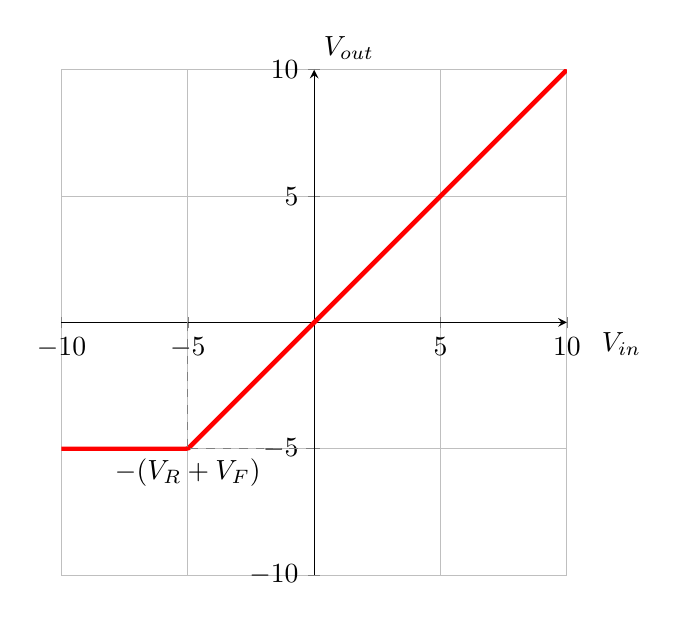
\begin{tikzpicture}
			\begin{axis}[
				axis lines=middle,
				xlabel={$V_{in}$},
				ylabel={$V_{out}$},
				xmin=-10, xmax=10,
				ymin=-10, ymax=10,
				grid=both,
				width=8cm, height=8cm,
				xlabel style={at={(ticklabel* cs:1.05)}, anchor=north west},
				ylabel style={at={(ticklabel* cs:1)}, anchor=south west},
				%title={\textbf{Biased Negative ($V_R = -2\text{V}$)}}
				]
				% Clipping behavior
				\addplot[ultra thick, red, domain=-10:10, samples=200] {max(x, -5)};
				% Reference Guide Lines
				\draw[dashed, gray] (axis cs:-5,0) -- (axis cs:-5,-5) node[below, black] {$-(V_R+V_F)$};
				\draw[dashed, gray] (axis cs:0,-5) -- (axis cs:-5,-5);
			\end{axis}
		\end{tikzpicture}
		\caption{Transfer characteristics of biased negative clippers}
		\label{fig:TransferCharBiasNegClipper}
	\end{subfigure}
	\caption{Biased negative clipper: Waveforms and transfer characteristics}	
\end{figure}

\begin{figure}[htbp]
	\centering
	\begin{subfigure}{0.75\textwidth}
		\centering
		\begin{tikzpicture}
			\begin{groupplot}[
				group style={
					group size=1 by 2,
					vertical sep=1.5cm,
				},
				width=10cm, height=5cm,
				axis lines=middle,
				xmin=-0.3, xmax=4.5,
				ymin=-6, ymax=6,
				xtick={0,2,4},
				xticklabels={$0$,$T$,$2T$},
				domain=0:4,
				samples=200,
				clip=false,
				]
				
				% ---------- PANEL 1: INPUT ----------
				\nextgroupplot[
				ylabel={$v_{in}(t)$},
				ylabel style={
					at={(axis description cs:0,1)},  % top-left corner of the axis
					anchor=south,
					rotate=0,
				},
				ytick={5,-5},
				yticklabels={$V_m$,$-V_m$},
				]
				\addplot[thick, blue] {5*sin(deg(pi*x))};
				\draw[dashed, gray] (axis cs:0,5) -- (axis cs:4,5);
				\draw[dashed, gray] (axis cs:0,-5) -- (axis cs:4,-5);
				
				% ---------- PANEL 2: OUTPUT (clipped) ----------
				\nextgroupplot[
				ylabel={$v_{out}(t)$},
				ylabel style={
					at={(axis description cs:0,1)},  % top-left corner of the axis
					anchor=south,
					rotate=0,
				},
				ytick={2,5},
				yticklabels={$+(V_R-V_F)\ \text{V}$,$V_m$},
				samples=400,
				]
				\addplot[thick, red] {max(2, 5*sin(deg(pi*x)))};
				\draw[dashed, gray] (axis cs:0,-3) -- (axis cs:4,-3);
				\draw[dashed, gray] (axis cs:0,5) -- (axis cs:4,5);
			\end{groupplot}
		\end{tikzpicture}
		\caption{Biased negative clipper waveforms with positive clipping level (polarity of $V_R$ reversed in Fig.~\ref{fig:biasedNegClipperDc})\footnote{Reversal of Zener polarity in Fig.~\ref{fig:biasedNegClipperZener} to achieve the same results is not possible. Can you think why?}}
		\label{fig:biasedNegClipperWavesPosLevel}
	\end{subfigure}
	\begin{subfigure}{0.75\textwidth}
		\centering
		% --- BIASED NEGATIVE (POSITIVE LEVEL +2V) ---
		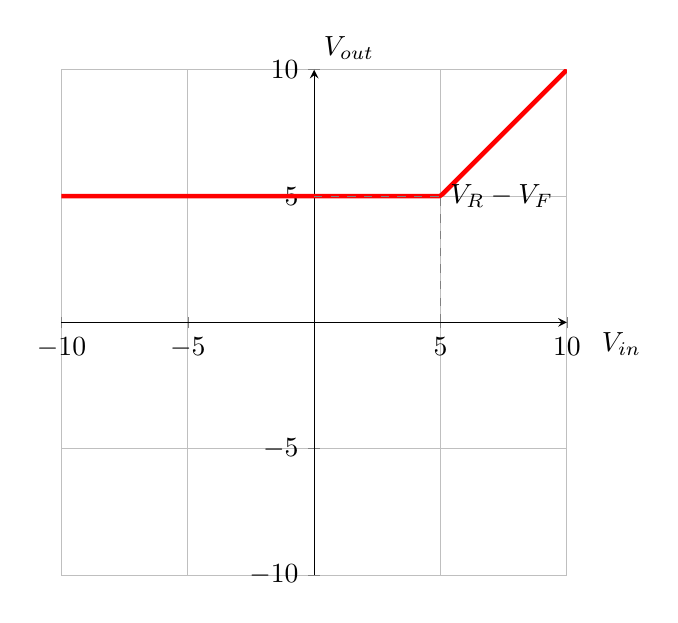
\begin{tikzpicture}
			\begin{axis}[
				axis lines=middle,
				xlabel={$V_{in}$},
				ylabel={$V_{out}$},
				xmin=-10, xmax=10,
				ymin=-10, ymax=10,
				grid=both,
				width=8cm, height=8cm,
				xlabel style={at={(ticklabel* cs:1.05)}, anchor=north west},
				ylabel style={at={(ticklabel* cs:1)}, anchor=south west},
				%title={\textbf{Biased Negative ($V_R = +2\text{V}$)}}
				]
				% Clipping behavior
				\addplot[ultra thick, red, domain=-10:10, samples=200] {max(x, 5)};
				% Reference Guide Lines
				\draw[dashed, gray] (axis cs:5,0) -- (axis cs:5,5) node[ right, black] {$V_R-V_F$};
				\draw[dashed, gray] (axis cs:0,5) -- (axis cs:5,5);
			\end{axis}
		\end{tikzpicture}
		\caption{Transfer characteristics of biased negative clippers: clipping at positive level}
		\label{fig:TransferCharBiasNegClipperPosLevel}
	\end{subfigure}
	\caption{Biased negative clipper with positive level: Waveforms and transfer characteristics}	
\end{figure}
\clearpage
\subsubsection{Slicer/Double Clipper}
\begin{figure}[hbtp]
	\centering
	\begin{subfigure}{0.42\textwidth}
		\centering
		\begin{circuitikz}[american, scale=1.0, line width=0.8pt]
			\draw
			(0,0) to[sinusoidal voltage source, l=$v_{in}(t)$] (0,3)
			(0,3) to[R, l=$R$, *-*] (2.8,3)
			(2.8,3) to[short] (5,3)
			(2.8,3) to[D, l=$D_1$, *-] (2.8,1.8)
			(2.8,1.8) to[battery1, l=$V_{R1}$, *-*] (2.8,0)
			(2.8,0) to[short] (0,0)
			(4.4,3) to[D, l=$D_2$, invert, *-*] (4.4,1.8)
			(4.4,1.8) to[battery1, l=$V_{R2}$, invert] (4.4,0)
			(4.4,0) to[short, -*] (0,0)
			;
			\draw (4.4,3) to[short, -o] (6,3) node[right]{$v_{out}(t)$};
			\draw (4.4,0) to [short, -o] (6,0) node[right]{};
			\draw (0,0) node[ground]{};
			\draw (5.8,3) to [R, l=$R_L$, *-*] (5.8,0);
		\end{circuitikz}
		\caption{Slicer Circuit}
		\label{fig:double_clipper}
	\end{subfigure}
	\hfill
	\begin{subfigure}{0.45\textwidth}
		\centering
		\begin{tikzpicture}
			\begin{groupplot}[
				group style={
					group size=1 by 2,
					vertical sep=1.0cm,
				},
				width=6cm, height=3.5cm,
				axis lines=middle,
				xmin=-0.3, xmax=4.5,
				ymin=-6, ymax=6,
				xtick={0,2,4},
				xticklabels={$0$,$T$,$2T$},
				domain=0:4,
				samples=200,
				clip=false,
				]
				
				% ---------- PANEL 1: INPUT ----------
				\nextgroupplot[
				ylabel={$v_{in}(t)$},
				ylabel style={
					at={(axis description cs:0,1)},  % top-left corner of the axis
					anchor=south,
					rotate=0,
				},
				ytick={5,-5},
				yticklabels={$V_m$,$-V_m$},
				]
				\addplot[thick, blue] {5*sin(deg(pi*x))};
				\draw[dashed, gray] (axis cs:0,5) -- (axis cs:4,5);
				\draw[dashed, gray] (axis cs:0,-5) -- (axis cs:4,-5);
				
				% ---------- PANEL 2: OUTPUT (clipped) ----------
				\nextgroupplot[
				ylabel={$v_{out}(t)$},
				ylabel style={
					at={(axis description cs:0,1)},  % top-left corner of the axis
					anchor=south,
					rotate=0,
				},
				ytick={-3,3},
				yticklabels={$-(V_{R2}+V_F)\ \text{V}$,$(V_{R1}+V_F)\ \text{V}$},
				samples=400,
				]
				\addplot[thick, red, samples=200] {max(-3, min(3, 5*sin(deg(pi*x))))};
				\draw[dashed, gray] (axis cs:0,-3) -- (axis cs:4,-3);
				\draw[dashed, gray] (axis cs:0,3) -- (axis cs:4,3);
			\end{groupplot}
		\end{tikzpicture}
		\caption{Input and output waveforms}
		\label{fig:slicerWaves}
	\end{subfigure}
	\caption{Slicer circuit and waveforms}
	\label{fig:slicer}
\end{figure}
%\clearpage
\subsection{Clamping Circuits}
\begin{figure}[htbp]
	\centering
	\begin{subfigure}{0.4\textwidth}
		\centering
		\begin{circuitikz}[american, scale=0.8, line width = 0.85pt]
			\draw
			(0,0) to[sinusoidal voltage source, l=$v_{in}(t)$] (0,3)
			(0,3) to[cC, name = C, l=$C$, *-*] (2,3)
			(2,3) to[short] (3.5,3)
			(2,3) to[D, l=$D$, *-, mirror] (2,0)
			(2,0) to[short, -*] (0,0)
			(3.5,3) to[R, l=$R_L$] (3.5,0)
			(3.5,0) to [short, -*] (2,0);	
			\node [above left=1pt] at (C.left){\small $+$};	
		\end{circuitikz}
		\caption{Negative clamper circuit.}
		\label{fig:neg_clamper}
	\end{subfigure}
	\hfill
	\begin{subfigure}{0.4\textwidth}
		\centering
		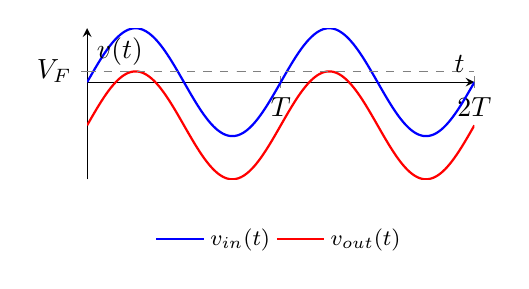
\begin{tikzpicture}
			\begin{axis}[
				width=6.5cm, height=3.5cm,
				xlabel={$t$}, 
				ylabel={$v(t)$},
				ylabel style={
					at={(axis description cs:0,1)},  % top-left corner of the axis
					anchor=south,
					rotate=90,
				},
				axis lines=middle,
				ymin=-4.5, ymax=2.5,
				xtick={0,1,2},
				xticklabels={$0$,$T$,$2T$},
				ytick={0.5},
				yticklabels={$V_F$},
				domain=0:2, samples=200,
				legend style={draw=none, font=\footnotesize, at={(0.5,-0.25)}, anchor=north, legend columns=2}
				]
				\addplot[blue, thick] {2.5*sin(360*x)};
				\addlegendentry{$v_{in}(t)$}
				\addplot[red, thick] {2.5*sin(360*x) - 2.5 + 0.5};
				\addlegendentry{$v_{out}(t)$}
				\addplot[gray, dashed] {0.5};
			\end{axis}
		\end{tikzpicture}
		\caption{Input and output waveforms for the negative clamper.}
		\label{fig:negWave_clamper}
	\end{subfigure}
	\caption{Negative Clamper: Circuit and waveforms}
\end{figure}
\begin{figure}[htbp]
	\centering
	\begin{subfigure}{0.4\textwidth}
		\centering
		\begin{circuitikz}[american, scale=0.8, line width=0.85pt]
			\draw
			(0,0) to[sinusoidal voltage source, l=$v_{in}(t)$] (0,3)
			(0,3) to[cC, name = C, l=$C$, invert, *-*] (2,3)
			(2,3) to[short] (3.5,3)
			(2,3) to[D, l=$D$, *-, invert] (2,0)
			(2,0) to[short, -*] (0,0)
			(3.5,3) to[R, l=$R_L$] (3.5,0)
			(3.5,0) to [short, -*] (2,0);	
			\node [above right=1pt] at (C.left){\small $+$};	
		\end{circuitikz}
		\caption{Positive clamper circuit (diode polarity reversed with respect to Figure~\ref{fig:neg_clamper}).}
		\label{fig:pos_clamper}
	\end{subfigure}
	\hfill
	\begin{subfigure}{0.4\textwidth}
		\centering
		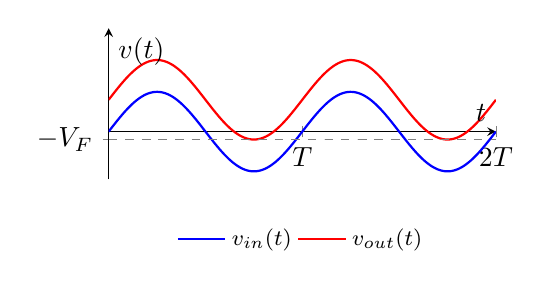
\begin{tikzpicture}
			\begin{axis}[
				width=6.5cm, height=3.5cm,
				xlabel={$t$}, 
				ylabel={$v(t)$},
				ylabel style={
					at={(axis description cs:0,1)},  % top-left corner of the axis
					anchor=south,
					rotate=90,
				},
				axis lines=middle,
				ymin=-3, ymax=6.5,
				xtick={0,1,2},
				xticklabels={$0$,$T$,$2T$},
				ytick={-0.5},
				yticklabels={$-V_F$},
				domain=0:2, samples=200,
				legend style={draw=none, font=\footnotesize, at={(0.5,-0.25)}, anchor=north, legend columns=2}
				]
				\addplot[blue, thick] {2.5*sin(360*x)};
				\addlegendentry{$v_{in}(t)$}
				\addplot[red, thick] {2.5*sin(360*x) + 2.5 - 0.5};
				\addlegendentry{$v_{out}(t)$}
				\addplot[gray, dashed] {-0.5};
			\end{axis}
		\end{tikzpicture}
		\caption{Input and output waveforms for the positive clamper.}
		\label{fig:posWaveClamper}
	\end{subfigure}
	\caption{Positive clamper: Circuit and waveforms}
\end{figure}
\clearpage
\begin{notebox}
	While preparing the lab-report, circuit diagrams shall contain proper labels for the components, including the component part numbers (such as 1N4001), and values/parameters (example: $10\ V_{pp}$, Sine, 100 Hz, for the source; $R_1$, $1\ \text{k}\Omega$, etc.).
\end{notebox}	
%\begin{notebox}
%	Show the actual design in the lab report instead of reproducing the design procedure.
%\end{notebox}
\section{Experiment Procedure}

\begin{enumerate}[label=\arabic*.]
	\item Assemble the shunt positive clipper of Figure~\ref{fig:ShuntPosClipperCkt} on the breadboard. Set the function generator to a sine wave of frequency $1\,\text{kHz}$ and amplitude $10\,\text{V}_{pp}$. 
	\item Connect DSO CH1 to $v_{in}$ and CH2 to $v_{out}$, with a common ground. Display both waveforms simultaneously and sketch/record them.
	\item Replace the shunt positive clipper with the shunt negative clipper. (Figure~\ref{fig:ShuntNegClipperCkt}). Record $v_{in}$ and $v_{out}$, and measure the clipping level from the DSO screen using the horizontal cursors.
	\item Repeat for the biased clipper (Figure~\ref{fig:biased_clipper}) for at least two values of $V_R$, and the double clipper (Figure~\ref{fig:double_clipper}). (\emph{Note that the peak of the selected input waveform is to be higher than the clipping level for the case of biased clippers}).
	\item For each clipper configuration, tabulate the theoretically expected and experimentally measured clipping levels.
	\item Assemble the negative clamper (Figure~\ref{fig:neg_clamper}) using the design values of $R_L$ and $C$ computed in the Design Procedure. Apply the same sine wave and record $v_{in}$ and $v_{out}$ on the DSO, noting the DC shift and any tilt/sag in the output.
	\item Repeat for the positive clamper (Figure~\ref{fig:pos_clamper}).
	\item For each clamper, measure $V_{out,max}$ and $V_{out,min}$ using DSO cursors and compare with Equations~\eqref{eq:neg_clamp}--\eqref{eq:pos_clamp}.
	\item Vary the input frequency (e.g., to $100\,\text{Hz}$) while keeping $R_L C$ fixed, and observe/record the effect on clamper output tilt. Explain the observation.
\end{enumerate}

\section{Precautions}
\begin{itemize}
	\item Observe correct diode polarity while assembling each circuit; an inverted diode produces the mirror-image (and often misleading) result.
	\item Do not exceed the diode's maximum forward current or reverse voltage ratings (Important if you are using a step-down transformer to give the input signal (50 Hz), instead of a function generator).
	\item Ensure a common ground between the function generator and both DSO channels.
%	\item For clamping circuits, allow a few cycles for the capacitor to reach steady-state charge before recording the output.
	\item Electrolytic capacitors, if used, connect with correct polarity as per the expected DC level at that node.
\end{itemize}
\section{Expected Waveforms}
The sample waveforms for the clipping circuits are as shown in Figs.~\ref{fig:wavePosClipper}, \ref{fig:NegClipperWaves},\ref{fig:biasedPosClipperWaves}, \ref{fig:biasedNegClipperWaves} and \ref{fig:slicerWaves}. The waveforms for the clamping circuits are as shown in Figs.~\ref{fig:negWave_clamper}, ~\ref{fig:posWaveClamper}. When recording waveforms, note down all the salient points/features of the waveforms, such as voltage/time details.

\section{Observation Tables}
The observation table for the clipping circuits is given in Table~\ref{tab:ObsClippers}. Use Table~\ref{tab:ObsClampers} to tabulate the Clamper circuit observations.
\begin{table}[ht!]
	\centering
	\begin{tabular}{@{}lccccc@{}}
		\toprule
		Circuit & $V_{clip}$ (theory) & $V_{clip}$ (measured) & \% Error \\
		\midrule
		Shunt positive clipper &  &  &  \\
		Shunt negative clipper &  &  &  \\
		Biased positive clipper ($V_{R1}$) &  &  &  \\
		Biased megative clipper ($V_{Z}$) &  &  &  \\
		Double clipper (upper level) &  &  &  \\
		Double clipper (lower level) &  &  &  \\
		\bottomrule
	\end{tabular}
	\caption{Clipping circuits: theoretical vs. measured clipping levels.}
	\label{tab:ObsClippers}
\end{table}

\begin{table}[ht!]
	\centering
	\begin{tabular}{@{}lcccc@{}}
		\toprule
		Circuit & $V_{out,max}$ (theory) & $V_{out,max}$ (meas.) & $V_{out,min}$ (theory) & $V_{out,min}$ (meas.) \\
		\midrule
		Negative clamper &  &  &  &  \\
		Positive clamper &  &  &  &  \\
		\bottomrule
	\end{tabular}
	\caption{Clamping circuits: theoretical vs. measured output extremes.}
	\label{tab:ObsClampers}
\end{table}
\section{Results}
\begin{enumerate}
	\item The diode-based clipping circuits with and without external bias are set-up and the output waveforms were studied. 
	\item The diode-based clamping circuits were set-up and the waveforms were studied.
\end{enumerate}


\begin{explorebox}
	Experiment with higher frequency signals. What do you observe? Can you explain why circuit performance is not as expected at higher frequencies?
\end{explorebox}
\section{Questions}
\begin{enumerate}[label=Q\arabic*.]
	\item Distinguish between series and shunt clipper configurations in terms of output impedance and loading effects.
	\item Derive the expression for the clipping level of the biased clipper of Figure~\ref{fig:biased_clipper} in terms of $V_R$ and $V_F$.
	\item Why must the time constant $R_L C$ of a clamper be much greater than the period of the input waveform? What happens if $R_L C$ is comparable to $T$?
	\item Sketch the output waveform of the double clipper (Figure~\ref{fig:double_clipper}) for an input triangular wave of amplitude greater than $(V_{R1}+V_{R2}+2V_F)$.
	\item A clamper is required to shift a $10\,\text{V}_{pp}$, $1\,\text{kHz}$ sine wave so that its output never goes negative. Design suitable values of $R_L$ and $C$, assuming a maximum permissible sag of $2\%$.
	\item Explain why a clipper is sometimes called a \emph{limiter} and give one practical application each of a clipper and a clamper in electronic systems.
	\item Why do clipper circuits do not perform as intended when diodes like 1N4001 are used, at higher frequencies, such as 50 kHz?
\end{enumerate}